\documentclass[tikz,border=12pt]{standalone}
\usepackage[utf8]{inputenc}
\usepackage[T1]{fontenc}
\usepackage{amsmath,amssymb}
\usepackage{tikz}
\usepackage{pgfplots}
\pgfplotsset{compat=1.18}
\usepgfplotslibrary{groupplots}
\usetikzlibrary{arrows.meta,positioning,calc,backgrounds}

% V6 pastel-first palette
\definecolor{CoreNavy}{RGB}{72,92,120}
\definecolor{MutedBlue}{RGB}{104,132,164}
\definecolor{MutedRust}{RGB}{174,112,96}
\definecolor{MutedTeal}{RGB}{92,146,142}
\definecolor{PaleBlue}{RGB}{235,241,247}
\definecolor{PaleTeal}{RGB}{232,244,242}
\definecolor{PalePeach}{RGB}{248,238,231}
\definecolor{PaleRose}{RGB}{247,235,235}
\definecolor{SoftGray}{RGB}{244,245,246}
\definecolor{MidGray}{RGB}{153,160,168}
\definecolor{Ink}{RGB}{40,45,52}

\tikzset{
  module/.style={
    draw=CoreNavy,
    fill=SoftGray,
    line width=0.8pt,
    rounded corners=2mm,
    inner xsep=3.5mm,
    inner ysep=2.2mm,
    font=\sffamily\footnotesize,
    text=Ink,
    align=center
  }
}

\begin{document}
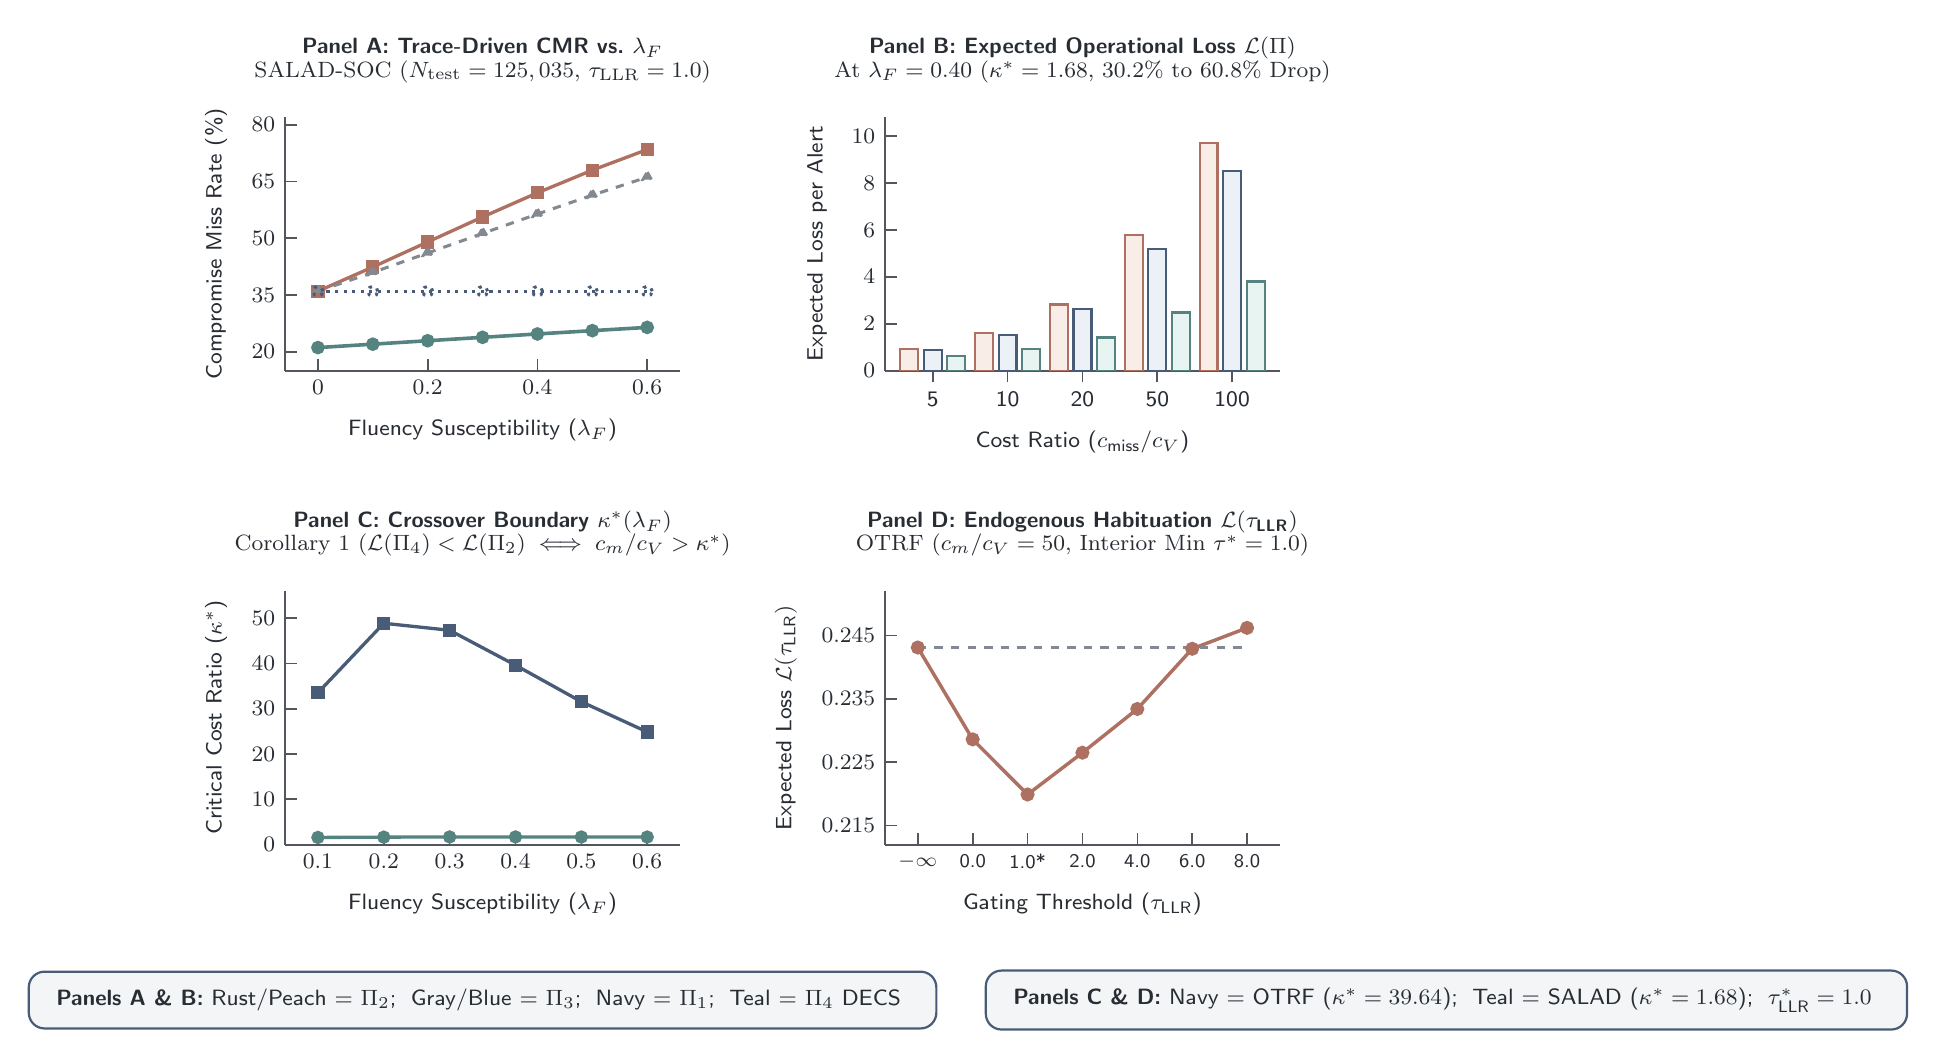
\begin{tikzpicture}[node distance=12mm and 14mm]

\begin{groupplot}[
  group style={
    group size=2 by 2,
    horizontal sep=26mm,
    vertical sep=28mm
  },
  width=66mm,
  height=48mm,
  grid=none,
  axis lines*=left,
  axis line style={draw=Ink!80, line width=0.7pt},
  tick style={draw=Ink!80, line width=0.6pt},
  tick label style={font=\sffamily\footnotesize, text=Ink},
  ylabel style={font=\sffamily\footnotesize, text=Ink, yshift=2pt},
  xlabel style={font=\sffamily\footnotesize, text=Ink, yshift=-2pt},
  title style={font=\sffamily\footnotesize\bfseries, text=Ink, align=center, yshift=3pt}
]

% Panel A: SALAD-SOC Trace-Driven CMR vs Fluency Susceptibility lambda_F
\nextgroupplot[
  title={Panel A: Trace-Driven CMR vs.\ $\lambda_F$\\[-1pt]\normalfont\footnotesize SALAD-SOC ($N_{\text{test}}=125,035$, $\tau_{\text{LLR}}=1.0$)},
  xlabel={Fluency Susceptibility ($\lambda_F$)},
  ylabel={Compromise Miss Rate (\%)},
  ymin=15, ymax=82,
  ytick={20,35,50,65,80},
  xtick={0.0,0.2,0.4,0.6}
]
% Pi_2: Unassisted Fluent
\addplot[color=MutedRust, line width=1.2pt, mark=square*, mark size=1.8pt] coordinates {
  (0.0,36.00) (0.1,42.40) (0.2,49.02) (0.3,55.63) (0.4,62.02) (0.5,68.01) (0.6,73.46)
};
% Pi_3: Static Banner
\addplot[color=MidGray!80!Ink, line width=1.1pt, dashed, mark=triangle*, mark size=1.8pt] coordinates {
  (0.0,36.00) (0.1,40.97) (0.2,46.10) (0.3,51.28) (0.4,56.41) (0.5,61.40) (0.6,66.15)
};
% Pi_1: Disfluent Baseline
\addplot[color=CoreNavy, line width=1.1pt, dotted, mark=o, mark size=1.8pt] coordinates {
  (0.0,36.00) (0.1,36.00) (0.2,36.00) (0.3,36.00) (0.4,36.00) (0.5,36.00) (0.6,36.00)
};
% Pi_4: Selective DECS
\addplot[color=MutedTeal!85!Ink, line width=1.3pt, mark=*, mark size=1.8pt] coordinates {
  (0.0,21.10) (0.1,22.00) (0.2,22.91) (0.3,23.81) (0.4,24.70) (0.5,25.58) (0.6,26.44)
};

% Panel B: Expected Loss Reduction Across Cost Ratios c_miss / c_V
\nextgroupplot[
  title={Panel B: Expected Operational Loss $\mathcal{L}(\Pi)$\\[-1pt]\normalfont\footnotesize At $\lambda_F=0.40$ ($\kappa^*=1.68$, $30.2\%$ to $60.8\%$ Drop)},
  xlabel={Cost Ratio ($c_{\text{miss}} / c_V$)},
  ylabel={Expected Loss per Alert},
  ybar=2pt,
  ymin=0, ymax=10.8,
  ytick={0,2,4,6,8,10},
  symbolic x coords={CR5,CR10,CR20,CR50,CR100},
  xtick={CR5,CR10,CR20,CR50,CR100},
  xticklabels={5,10,20,50,100},
  xticklabel style={align=center, font=\sffamily\footnotesize, text=Ink},
  enlarge x limits=0.16
]
% Pi_2: Unassisted Fluent
\addplot[
  draw=MutedRust,
  line width=0.8pt,
  fill=PalePeach,
  bar width=6.5pt
] coordinates {
  (CR5,0.9099) (CR10,1.6104) (CR20,2.8201) (CR50,5.7700) (CR100,9.6860)
};
% Pi_3: Static Banner
\addplot[
  draw=CoreNavy,
  line width=0.8pt,
  fill=PaleBlue,
  bar width=6.5pt
] coordinates {
  (CR5,0.8855) (CR10,1.5302) (CR20,2.6171) (CR50,5.1916) (CR100,8.5188)
};
% Pi_4: Selective DECS
\addplot[
  draw=MutedTeal!85!Ink,
  line width=0.8pt,
  fill=PaleTeal,
  bar width=6.5pt
] coordinates {
  (CR5,0.6355) (CR10,0.9364) (CR20,1.4125) (CR50,2.4782) (CR100,3.7995)
};

% Panel C: Corollary 1 Critical Cost-Ratio Crossover kappa*(lambda_F)
\nextgroupplot[
  title={Panel C: Crossover Boundary $\kappa^*(\lambda_F)$\\[-1pt]\normalfont\footnotesize Corollary 1 ($\mathcal{L}(\Pi_4)<\mathcal{L}(\Pi_2) \iff c_m/c_V > \kappa^*$)},
  xlabel={Fluency Susceptibility ($\lambda_F$)},
  ylabel={Critical Cost Ratio ($\kappa^*$)},
  ymin=0, ymax=56,
  ytick={0,10,20,30,40,50},
  xtick={0.1,0.2,0.3,0.4,0.5,0.6}
]
% OTRF kappa*
\addplot[color=CoreNavy, line width=1.2pt, mark=square*, mark size=1.8pt] coordinates {
  (0.1,33.54) (0.2,48.90) (0.3,47.35) (0.4,39.64) (0.5,31.56) (0.6,24.88)
};
% SALAD-SOC kappa*
\addplot[color=MutedTeal!85!Ink, line width=1.2pt, mark=*, mark size=1.8pt] coordinates {
  (0.1,1.57) (0.2,1.64) (0.3,1.68) (0.4,1.68) (0.5,1.67) (0.6,1.66)
};

% Panel D: Unified Endogenous Habituation U-Shaped Curve L(tau_LLR) on OTRF
\nextgroupplot[
  title={Panel D: Endogenous Habituation $\mathcal{L}(\tau_{\text{LLR}})$\\[-1pt]\normalfont\footnotesize OTRF ($c_m/c_V=50$, Interior Min $\tau^*=1.0$)},
  xlabel={Gating Threshold ($\tau_{\text{LLR}}$)},
  ylabel={Expected Loss $\mathcal{L}(\tau_{\text{LLR}})$},
  ymin=0.212, ymax=0.252,
  ytick={0.215,0.225,0.235,0.245},
  yticklabel style={/pgf/number format/fixed, /pgf/number format/precision=3},
  symbolic x coords={Inf,T0,T1,T2,T4,T6,T8},
  xtick={Inf,T0,T1,T2,T4,T6,T8},
  xticklabels={$-\infty$,0.0,1.0*,2.0,4.0,6.0,8.0},
  xticklabel style={align=center, font=\sffamily\scriptsize, text=Ink}
]
\addplot[color=MutedRust, line width=1.25pt, mark=*, mark size=1.9pt] coordinates {
  (Inf,0.2431) (T0,0.2286) (T1,0.2199) (T2,0.2265) (T4,0.2334) (T6,0.2429) (T8,0.2462)
};
% Static Pi_3 reference line
\addplot[color=MidGray!80!Ink, line width=0.9pt, dashed] coordinates {
  (Inf,0.2431) (T8,0.2431)
};

\end{groupplot}

% Relative summary nodes below panels
\node[module, below=16mm of group c1r2.south] (note_a) {
  \textbf{Panels A \& B:} Rust/Peach = $\Pi_2$;\; Gray/Blue = $\Pi_3$;\; Navy = $\Pi_1$;\; Teal = $\Pi_4$ DECS
};
\node[module, right=6mm of note_a] (note_b) {
  \textbf{Panels C \& D:} Navy = OTRF ($\kappa^*=39.64$);\; Teal = SALAD ($\kappa^*=1.68$);\; $\tau^*_{\text{LLR}}=1.0$
};

\end{tikzpicture}
\end{document}
